\chapter{Diseño e implementación}
\label{cap:diseñoeimplementación}

%Hacer intro de esta sección, supongo que cuando esté algo más hecho será más fácil hacerla.

Hemos planteado la aplicación como un modelo cliente-servidor, en la que el servidor se encargará de ejecutar el programa que lleve a cabo todos los cálculos y se los proporcionará al cliente (dispositivo móvil) cuando este lo solicite. De esta manera, nuestro programa estará mejor organizado, será mas rápido y evitaremos que nuestro dispositivo móvil se quede sin batería en el cálculo de datos. A continuación detallaremos el diseño y la implementación tanto del cliente como del servidor.


\section{Servidor}
El servidor es una parte indispensable del proyecto ya que se encarga de realizar los cálculos más pesados para no sobrecargar al dispositivo móvil. Las principales tareas de las que se encarga son:
\begin{itemize}
	\item Permanecer a la escucha de cualquier cliente que solicite conexión.
	\item Solventar el posicionamiento del cliente conectado.
	\item Generar la mejor ruta (más corta y mejor adaptada) desde la posición actual hasta el destino indicado.
	\item Enviar la siguiente instrucción al cliente.	
\end{itemize} 

La aplicación servidor se divide en código java y los archivos .xml en los que se encuentra la información del edificio. Buena parte del código que los conforma ha sido reutilizado de trabajos anteriores, en concreto del proyecto \textit{Generador interactivo de instrucciones de guía sobre plataformas móviles} \citep{TFGguia} y del proyecto \textit{Sistema de guía por voz en interiores} \citep{TFGMariana}. Sin embargo se han introducido cambios notorios para el desarrollo de esta aplicación que comentaremos a continuación.

\subsection{Código java}
Para entender mejor la estructura de nuestro servidor, veamos las principales clases de las que se compone y su función. En la \ref{fig:diagServ} se puede ver el diagrama con las dependencias de cada una de ellas:

\begin{itemize}
	\item \textit{MainClienteAndroid}: como su propio nombre indica, es el \textit{Main} del servidor. Se hizo otra versión para probar el servidor sin necesidad de acceder a el mediante la aplicación móvil, es por ello que lleva el identificador de Ciente Android en el nombre. Esta clase se encarga de la conexión directa con el cliente, abre un \textit{ServerSocket} que queda a la espera de clientes y, una vez llegan, los atiende. Es decir, lee sus posiciones de origen y destino al que se quieren dirigir y devuelve la siguiente instrucción que deben seguir. Para ello se apoya en distintas clases que detallamos a continuación. 
	
	\item \textit{Edificio}: esta clase es muy importante, pues guarda la información relativa al mapeo: los cuadrantes y las estancias. En nuestro caso, estas últimas se corresponden con las plantas del edificio, para la Facultad de Informática tenemos dos estancias, la planta baja y la primera planta. Para llevar a cabo su objetivo, \textit{Edificio} lee el archivo edificio.xml que tiene como elementos las distintas plantas y de estas, carga la lista de cuadrantes y estancias con ayuda de la clase \textit{CargaXML}.
	
	\item \textit{Estancia} y \textit{Cuadrante}: sus propios nombres son muy descriptivos. La clase  \textit{Estancia} guarda la información de los cuadrantes que hay en cada planta y cuenta con funciones que permiten saber si un cuadrante está en una determinada estancia o añadir un cuadrante a una estancia. En el caso de la clase \textit{Cuadrante}, contamos con una serie de estructuras con las que almacenamos toda la información referente a estos, véase su identificador, el \textit{beacon} asociado, la información relevante de cada cuadrante, los metros que ocupa, la planta en la que está situado y, una de las cosas más importantes, con quién está conectado. 
	
	\item \textit{ListaCuadrantes}: esta clase constituye una parte muy importante ya que es la encargada de establecer la relación entre el identificador del cuadrante y el identificador del \textit{beacon} asociado, y de formar la matriz de adyacencia a partir de la información de conexión de cada cuadrante. Es aquí donde introducimos los pesos que tiene cada conexión en función de la dificultad que supone la misma para una persona con discapacidad visual. Veremos esto con más detalle en la Sección \ref{rutaEInst}. Esta clase también se encargará de obtener la lista de cuadrantes que conformarán la ruta de origen a destino mediante el algoritmo de \textit{Dijkstra}.
	
	\item \textit{Persona}: esta clase almacena la información referente a la ruta (lista de cuadrantes) que tiene que seguir el cliente para alcanzar el destino desde su posición origen. Para ello, llama a la función \textit{caminoConDijkstra} de la clase \textit{ListaCuadrantes}.
	
	\item \textit{GerenarRuta}: Es probablemente la clase más importante del servidor. Su objetivo es devolver la siguiente instrucción que debe seguir el cliente para completar la ruta. La función encargada que contiene toda la lógica relativa a este propósito es \textit{generar}. Esta función es una de las que más modificaciones ha sufrido con respecto a los trabajos predecesores, pues no solo la hemos adaptado para personas con discapacidad visual sino que también hemos incluido mucha complejidad al añadir cambios de planta y demás casuística que no estaba previamente incluida. La principal adaptación que hemos añadido es la de proporcionar instrucciones mucho más precisas e informadas. Por ejemplo: en lugar de finalizar la ruta con el mensaje ``Ha llegado a su destino.'', ahora se indica dónde está el destino dependiendo de la ruta que se haya seguido y la orientación del usuario. Podría ser: ``Su destino está a la derecha'' o a la izquierda, etc. Otra novedad es que la ruta incluye la posibilidad de informar anticipadamente sobre lo que el usuario se va a encontrar a su paso, como pueden ser pequeños escalones, baños, la cafetería, el despacho de Delegación de Alumnos, etc. Esto es fundamental pues además de dar seguridad al usuario le da la opción de tener una mejor idea global del espacio en el que se encuentra. Como ya hemos mencionado, otra ampliación que hemos introducido es la del cambio de planta. Para ello, hemos unido la planta baja y la primera planta por los cuadrantes correspondientes a los ascensores, permitiendo así tener origen y destino en plantas distintas. A pesar de que en la Facultad de Informática contamos con ascensores y escaleras, se ha supuesto que la ruta se seguirá por medio de los ascensores ya que de esta manera es más fácil el cambio de planta y, además, estos se encuentran adaptados con botones en \textit{braille}.
	
\end{itemize}


\begin{figure}[t]
	\centering
	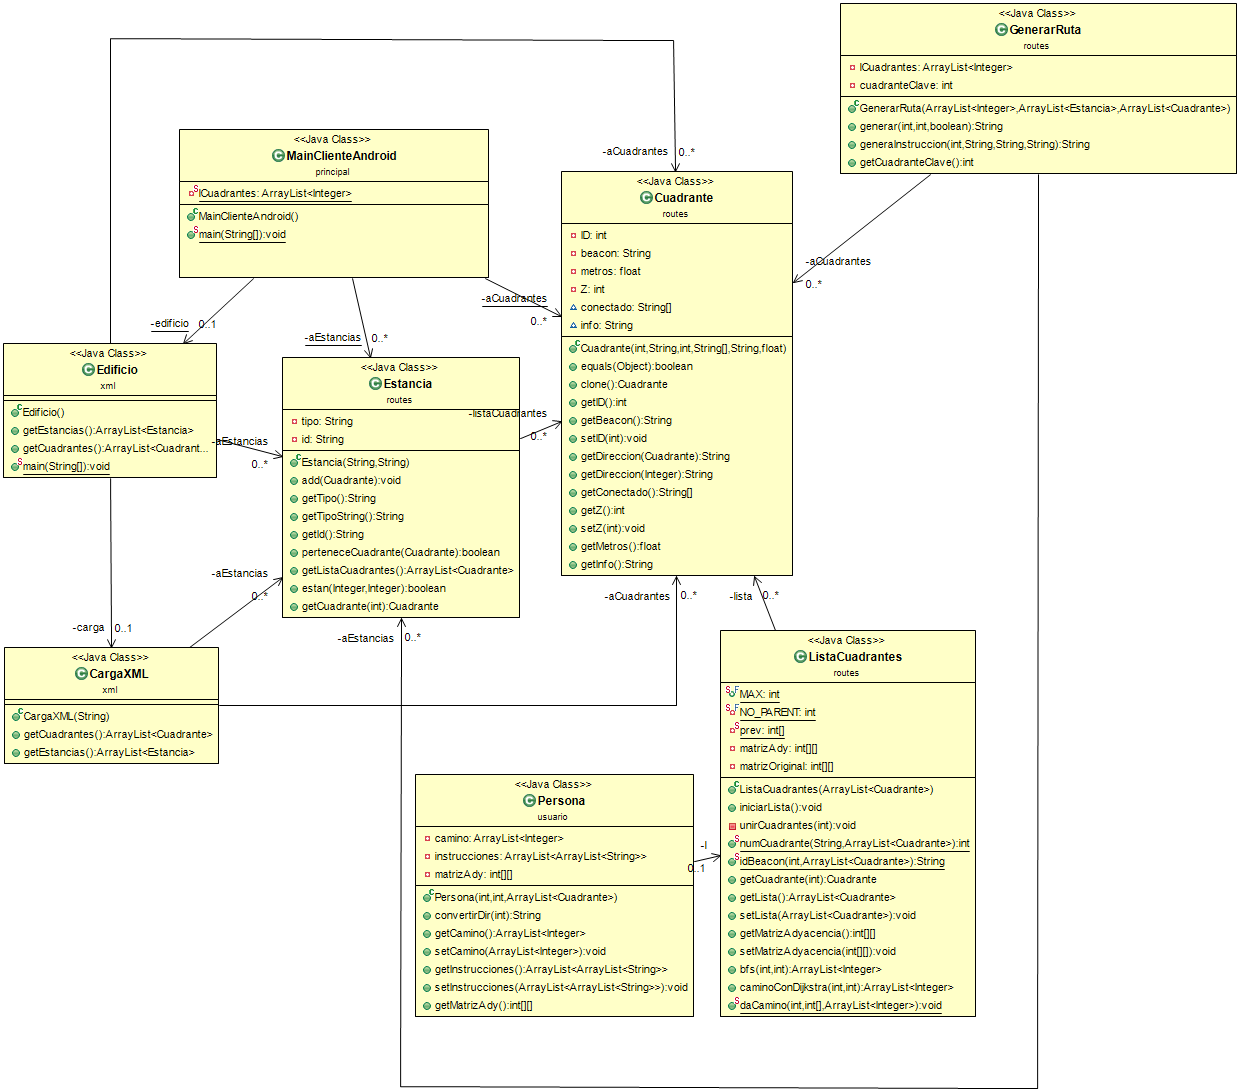
\includegraphics[width=1.1\textwidth]{Imagenes/Capitulo4/diagramServer}
	\caption{Diagrama de las clases principales del servidor.}
	\label{fig:diagServ}
\end{figure}


\subsection{Cálculo de la ruta óptima}
\label{rutaEInst}

Una vez que el mapeo del edificio y el posicionamiento del usuario están resueltos es hora de comenzar a trabajar en la obtención de la ruta más adecuada. El mapeo que hemos visto en la Sección \ref{sec:mapeo} nos proporciona un grafo, en el que los cuadrantes son los nodos y las conexiones entre ellos, las aristas. Para su representación hemos empleado una matriz de adyacencia y de esta manera, el cálculo de la ruta más corta entre dos cuadrantes se reduce al algoritmo de \textit{Dijkstra}.

Sin embargo, no debemos olvidar que nuestra aplicación tiene un usuario final muy concreto: personas con discapacidad visual. Es por ello que la ruta debe ser lo más sencilla posible, libre de obstáculos y otros elementos que puedan entorpecerles, por lo que en ocasiones la ruta óptima no coincide con la más corta. Tras hacer numerosas pruebas de distintas rutas, hemos detectado un ejemplo de ello: al comenzar en la puerta principal de la facultad y terminar en la puerta trasera de la cafetería, el algoritmo de \textit{Dijkstra} sugiere que el camino óptimo es acortar por detrás de conserjería (cuadrante 32) ya que es la ruta más corta pero no la óptima para una persona con discapacidad visual pues ese pasillo es más estrecho, la gente se suele aglomerar (están los ascensores, la gente continúa su camino a la cafetería, etc.) y cuenta con más giros. Por ello, hemos considerado que es más conveniente continuar la ruta por delante de Conserjería (cuadrantes 35-36-20) y luego girar a la izquierda (cuadrante 21). Para lograrlo hemos modificado la matriz de adyacencia, añadiendo más peso en aquellas conexiones que hemos considerado menos adecuadas. En este caso particular, a las conexiones entre los cuadrantes 31-32 y 32-22. De esta manera hacemos que el paso por el pasillo de los ascensores se limite únicamente al caso en el es estrictamente necesario pasar por allí, es decir, cuando se va a hacer un cambio de planta.


\subsection{Detalles técnicos del posicionamiento}

%COMPLETAR CUANDO ESTÉ EL CLIENTE Y VER ENTONCES DONDE SE VA A COLOCAR. En ese momento habrá que hablar tambien del cuadrante clave!!!

A diferencia de todos los proyectos previos de guía por la Facultad de Informática (comenzando por Avanti \citep{avanti}), el nuestro introduce una novedad notoria: los \textit{beacons}. Esto supone un gran cambio en el sistema de posicionamiento ya que eliminamos por completo la triangulación y nuestro servidor recibe información solo del \textit{beacon} más cercano al cliente. Es entonces cuando el servidor, a través de la clase \textit{ListaCuadrantes}, aproxima el cuadrante en el que se encuentra el cliente y saca la ruta a seguir.  %Veamos, de manera general, el funcionamiento del servidor cada vez que llega un nuevo cliente:

%\begin{enumerate}
%	\item El servidor recibe el beacon más cercano que tiene el cliente y el destino al que quiere ir. En base a eso reconoce los cuadrantes origen y destino.

%	\item Calcula la ruta óptima (en lo que sigue veremos a qué nos referimos con esto) que debe seguir el cliente desde el origen o posición actual del cliente para llegar al destino. 
%\end{enumerate}
CUANDO ESTE EL CLINTE COMPLETAMOS!!:
El cliente va llamando al servidor cuando actualiza su posición actual, de esta manera el servidor actualiza la ruta y genera la nueva instrucción. Una vez que la ruta ha finalizado, el servidor se lo indica al cliente con una instrucción de finalización. Véase, ``Su destino se encuentra a la derecha, el recorrido ha finalizado''.

\section{Cliente}